\documentclass[tikz,border=2pt]{standalone}
\usepackage{amsmath,amssymb}
\usepackage{pgfplots}
\pgfplotsset{compat=1.18}

\begin{document}
% Running averages of three simulated sequences of fair die rolls (n = 1..400): each individual
% path settles at the mean 3.5.
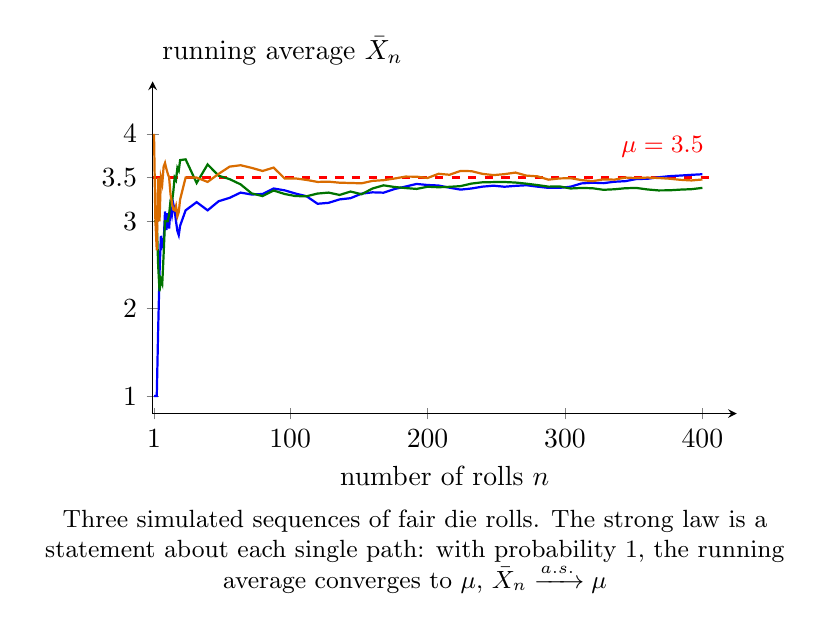
\begin{tikzpicture}
	\begin{axis}[
		axis lines=left, xmin=0, xmax=425, ymin=0.8, ymax=4.6,
		xtick={1,100,200,300,400}, ytick={1,2,3,3.5,4}, yticklabels={$1$,$2$,$3$,$3.5$,$4$},
		xlabel={number of rolls $n$}, ylabel={running average $\bar X_n$}, ylabel style={rotate=-90, anchor=south west, at={(axis description cs:0,1.02)}},
		width=9cm, height=5.8cm, clip=false
		]
		\draw[red, dashed, thick] (axis cs:0,3.5) -- (axis cs:410,3.5);
		\addplot[blue, thick] coordinates {(1,1.000) (2,1.000) (3,1.000) (4,1.750) (5,2.400) (6,2.833) (7,2.714) (8,2.750) (9,3.111) (10,2.900) (11,3.091) (12,2.917) (13,3.154) (14,3.071) (15,3.200) (16,3.125) (17,3.000) (18,2.889) (19,2.842) (20,2.950) (24,3.125) (32,3.219) (40,3.125) (48,3.229) (56,3.268) (64,3.328) (72,3.306) (80,3.312) (88,3.375) (96,3.354) (104,3.317) (112,3.286) (120,3.200) (128,3.211) (136,3.250) (144,3.264) (152,3.316) (160,3.331) (168,3.327) (176,3.369) (184,3.397) (192,3.427) (200,3.415) (208,3.409) (216,3.384) (224,3.362) (232,3.375) (240,3.396) (248,3.407) (256,3.395) (264,3.405) (272,3.412) (280,3.396) (288,3.382) (296,3.382) (304,3.395) (312,3.433) (320,3.441) (328,3.436) (336,3.452) (344,3.459) (352,3.483) (360,3.486) (368,3.503) (376,3.516) (384,3.523) (392,3.531) (400,3.538)};
		\addplot[green!45!black, thick] coordinates {(1,3.000) (2,3.000) (3,3.000) (4,2.500) (5,2.200) (6,2.333) (7,2.286) (8,2.625) (9,3.000) (10,3.000) (11,3.000) (12,3.083) (13,3.231) (14,3.214) (15,3.333) (16,3.500) (17,3.471) (18,3.611) (19,3.579) (20,3.700) (24,3.708) (32,3.438) (40,3.650) (48,3.521) (56,3.482) (64,3.422) (72,3.319) (80,3.288) (88,3.352) (96,3.312) (104,3.288) (112,3.286) (120,3.317) (128,3.328) (136,3.301) (144,3.340) (152,3.309) (160,3.375) (168,3.411) (176,3.392) (184,3.380) (192,3.370) (200,3.395) (208,3.389) (216,3.394) (224,3.402) (232,3.431) (240,3.446) (248,3.448) (256,3.449) (264,3.443) (272,3.430) (280,3.414) (288,3.396) (296,3.399) (304,3.375) (312,3.381) (320,3.378) (328,3.360) (336,3.366) (344,3.378) (352,3.381) (360,3.364) (368,3.353) (376,3.354) (384,3.362) (392,3.367) (400,3.382)};
		\addplot[orange!85!black, thick] coordinates {(1,4.000) (2,3.000) (3,2.667) (4,3.500) (5,3.000) (6,3.500) (7,3.429) (8,3.625) (9,3.667) (10,3.600) (11,3.545) (12,3.500) (13,3.308) (14,3.214) (15,3.133) (16,3.125) (17,3.176) (18,3.056) (19,3.105) (20,3.250) (24,3.500) (32,3.500) (40,3.450) (48,3.542) (56,3.625) (64,3.641) (72,3.611) (80,3.575) (88,3.614) (96,3.490) (104,3.490) (112,3.473) (120,3.450) (128,3.453) (136,3.441) (144,3.438) (152,3.434) (160,3.462) (168,3.470) (176,3.489) (184,3.511) (192,3.510) (200,3.495) (208,3.543) (216,3.532) (224,3.576) (232,3.573) (240,3.542) (248,3.528) (256,3.539) (264,3.557) (272,3.522) (280,3.514) (288,3.476) (296,3.490) (304,3.493) (312,3.471) (320,3.459) (328,3.479) (336,3.476) (344,3.500) (352,3.494) (360,3.500) (368,3.495) (376,3.487) (384,3.474) (392,3.467) (400,3.478)};
		\node[red, anchor=south east, font=\small] at (axis cs:408,3.62) {$\mu=3.5$};
	\end{axis}
	\node[anchor=north, font=\small, align=flush center, text width=9.6cm] at ([yshift=-2pt]current axis.outer south) {Three simulated sequences of fair die rolls. The strong law is a statement about each single path: with probability $1$, the running average converges to $\mu$, $\bar X_n\xrightarrow{a.s.}\mu$};
\end{tikzpicture}
\end{document}
